%% Full length research paper template
%% Created by Simon Hengchen and Nilo Pedrazzini for the Journal of Open Humanities Data (https://openhumanitiesdata.metajnl.com)

\documentclass{article}
\usepackage[english]{babel}
\usepackage[utf8]{inputenc}
\usepackage{johd}
\usepackage{amsmath}
\usepackage{svg}
\usepackage[margin=1cm]{caption}


\title{GPU optimization of Smith–Waterman algorithm}

\author{Samuele Allegranza \\
        \small Polytechnic University of Milan - GPU101 Course\\
}

\date{} %leave blank

\begin{document}

\maketitle

% 7 lines
\begin{abstract} 
\noindent This project involved the development of a CUDA program that  optimizes the execution of the Smith-Waterman algorithm on GPUs. A pair of approaches have been designed and tested in order to achieve the goal. The results presented significant advantages in terms of execution time, compared to the computation of the same algorithm on CPU. Parallelization of operations is the key behind these big improvements, a concept which is what the GPU architecture is based on. Presented solutions are good starting points for further improvements. \end{abstract}

\section{Introduction}
\noindent
The assigned project for the GPU101 course asked to implement a GPU optimized version of the Smith-Waterman algorithm, using C language with the CUDA API, which was the main subject of the lessons.\\

\noindent The Smith-Waterman algorithm performs local sequence alignment. It compares two different strings and computes the optimal alignment of them, applying a set of scoring rules. It is heavily used in bioinformatics to perform sequence alignment between two nucleotide or amino acid sequences, in order to find similarities between each other and understand if they are related.
This algorithm relies on dynamic programming, which finds the solution to a problem by breaking it down into simpler sub-problems and saving their solutions on memory.\\

\noindent The execution of this algorithm on a GPU could demonstrate significant performance improvements, provided that computation is well parallelized and resources are used efficiently. Fortunately, the nature of the Smith-Waterman algorithm allows a good degree of optimization.\\
The project has been developed on WSL (Windows Subsystem for Linux) and tested with an i5 6600k and a Nvidia GTX 1080.

\section{Methods}

Before diving into the project implementation is important to understand how the Smith-Waterman algorithm works. Technical details about the CUDA programming model are given too, which are essential for proper understanding of the proposed solutions.

\subsection{Smith-Waterman algorithm}
\noindent
The goal of the algorithm is to find the optimal alignment of two strings. In order to achieve this, it uses a scoring system. The scoring rules were given upfront, and can be customized correspondingly to the user needs.\\
Given two strings \(R, Q\) of lengths \(L\) (for simplicity, we assume they have same lengths), the matrices \(S\) and \(D\) are initialized with dimensions \((L \times L)\). \(S\) is the scoring matrix and \(D\) is the direction matrix. Every element \(S_{x,y}\) is computed calculating its corresponding score.\\
Firstly, string's characters \(R_x\) and \(Q_y\) are compared: if equal, \(c = P_{match}\), otherwise \(c = P_{mismatch}\), where \(P_{match}\) and \(P_{mismatch}\) are the predefined penalties for match or mismatch of characters. Then, the following equation is evaluated:
\[
S_{x,y} = \max\left\{\begin{array}{lr}
    S_{(x-1),(y-1)}+c, \\
    S_{(x-1),y} + P_{delete}, \\
    S_{x,(y-1)} + P_{insert}, \\
    0\\
    \end{array}\right\}
\]
where \(P_{insert}\) and \(P_{delete}\) are respectively insertion and deletion penalties.
The direction matrix \(D\) is also filled, pointing every score matrix's cell to the one from which the calculated score derives. If score is 0, then no direction is specified. So, every cell \(D_{x,y}\) will either point to the upper, left or upper-left cell, if specified.\\
After the score and the direction matrices are filled, the maximum score cell is identified, and from this one the \textit{backtracing} process is started. It consists in following the directions pointed out in the direction matrix, until a cell with score 0 is reached. In Figure \ref{fig_sw_example} is presented a complete example.

\begin{figure}[H]
\centering
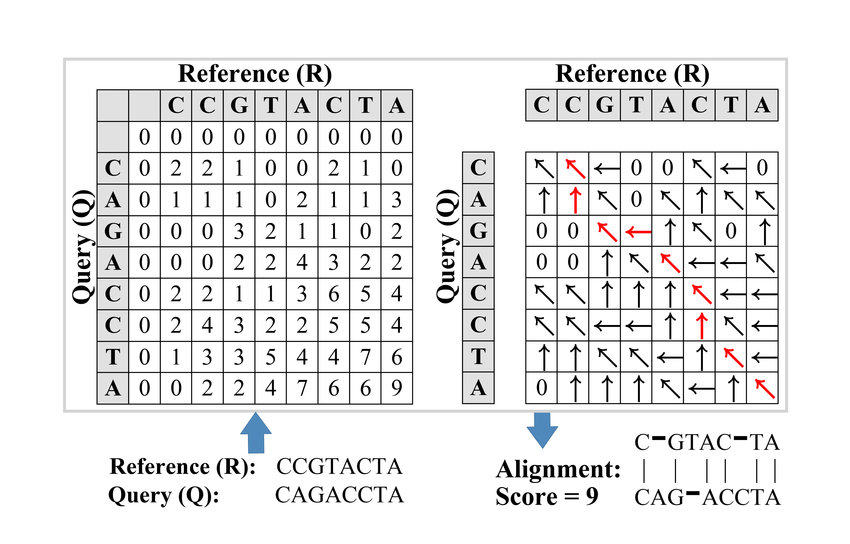
\includegraphics[scale=1.75]{images/sw_illustration.png}
\captionsetup{justification=centering}
\caption{\label{fig_sw_example}An example application of the Smith-Waterman algorithm applied to two strings \(R\) and \(Q\). On the left is illustrated the score matrix, and on the right the direction matrix. In red is visualized the traceback operation. Note that it has started from the maximum score cell. }
\end{figure}


\subsection{CUDA Programming model}
The project required a revisitation of the original algorithm described above, such that it could be executed on a GPU. The implementation of the Smith-Waterman algorithm for GPU execution was performed using CUDA, an API for C programming language, which gives to the programmer nearly-full controll of the GPU. It enables the development of algorithms in a friendly environment, with a good degree of abstraction from the hardware details. Nevertheless, a good understanding of the GPU architecture is required to be able to exploit the full potential of it.\\
The main characteristic of GPUs is that they have a much larger number of cores compared to ordinary CPUs. On the other hand, they are slower and have limitations regarding execution independence.
CUDA enables parallel execution of threads with a hierarchical approach: threads can be gropued in \textit{blocks} and the set of \textit{blocks} is called \textit{grid}. The way threads are grouped is decided by the programmer and has a lot of relevance regarding performance. 
Under the hood, CUDA bundles groups of threads with consecutive indexes into \textit{warps}, and each of them is executed on a single CUDA core. At run-time, warps will be assigned to the cores of a SM.\\
This style of execution is called SIMT (\textit{Single-instruction, Multiple Thread}), which is similar to SIMD (\textit{Single instruction, Multiple data}). The difference from SIMD is that threads are executed in parallel by a single instruction, and not data.\\
The solutions for this project have been tested with an Nvidia GTX 1080. It relies on the Pascal architecture, and more precisely mounts the GP104 chip. This card is equipped with 20 SMs, each warp carry 32 threads and the shared memory capacity per SM is 96KB.


\section{Implementation}\label{implementation}
The problem has been tackled with different approaches, which resulted in similar performance results. Before diving into the solutions, let's have a look at the opportunities and problems of trying to execute the Smith-Waterman algorithm on a GPU.\\

\noindent Constraints of the assigned project:
\begin{itemize}
    \item Strings to be processed have all the same length \(L\) (\textit{default}: \(L = 512\))
    \item The program has to execute Smith-Waterman on \(N\) pairs of strings (\textit{default}: \(N = 1000\))
    \item Score and direction matrices have dimensions \((L+1) \times (L+1)\). The first column and row of both are initialized to 0 and can be considered ``boundaries'' for the traceback, as well as a support for the computation of the first horizontal and vertical score lines.
\end{itemize}
The computationally intensive part of the Smith-Waterman algorithm is the calculation of both score and direction matrices. It's necessary to find a way to parallelize tasks in order to exploit the potential of GPUs.
Analyzing how the algorithm works, it is possible to identify that every cell \(C_{x,y}\) (distinction between score and direction cells isn't needed) is dependent on the value of 3 others: \(C_{x-1,y}\), \(C_{x,y-1}\) and \(C_{x-1,y-1}\). So, the parallelization of the computation of the matrices is limited by this ``constraint''.\\

Two different solutions have been developed for this project, which proved to be equally performing, even if they have radically different approaches for parallelization.

\subsection{``2-Threads'' solution}
\noindent
The first approach that came to mind was to split the load on two different threads \(T_1\) and \(T_2\) for each set of problems. For \(N\) problems that need to compute alignment of 2 strings each, the total amount of threads is \(2N\). So, \(N\) blocks of \(2\) threads each are allocated to compute all the alignments. This approach, in theory, isn't ideal, as allocating only 2 threads per block is not recommended due to constraints of the GPU architecture.\\
Once the kernel is started, \(T_1\) and \(T_2\) initialize the first row and column of score and direction matrices with 0s. Then, the computation starts.\\
\(T_1\) computes scores horizontally and \(T_2\) computes scores vertically, advancing diagonally downwards every time the current row/column is finished. This process is repeated \(L\) times. It's important to notice that load isn't perfectly distributed on each thread: for each iteration \(i\), the \(C_{i,i}\) cell (which corresponds to a cell of the main diagonal) needs to be computed by one of the two threads, while the other one has to idle until the score of it has been calculated. In the solution proposed, \(T_1\) handles the computation of cells on the main diagonal. Figure \ref{fig_2-threads} shows a graphical example.\\
While computing scores, each thread evaluates the maximum value found with its corresponding position. When all the cells of score and direction matrices are filled, the global maximum value between \(T_1\) and \(T_2\) is found and, finally, the traceback is performed by one of the threads.

\begin{figure}[H]
\centering
\includesvg[scale=0.65]{images/2-threads.svg}
\captionsetup{justification=centering}
\caption{\label{fig_2-threads}An example applying the ``2-Threads'' approach on its second iteration. In light-red, cells computed by \(T_1\) and in light-blue cells computed by \(T_2\). dark red and blue cells are currently processed.}
\end{figure}


\subsection{``\(L\)-Threads'' solution}
\noindent
The second approach aimed to improve the first one, by trying to maximize the number of parallel operations. Having every cell dependent on the left one, the upper one and the upper-left one, is understandable that, starting from the cell \(C_{0,0}\), is possible to compute them progressively in anti-diagonal direction. The peak number of parallel cells computed simultaneously is reached when the the anti-diagonal of the matrix is evaluated: it has \(L\) cells.\\
With this in mind, \(N\) blocks are allocated to solve a problem set each, and every block has a total of \(L\) threads \(T_0, T_1, ... , T_{L-1}\), which is equal to the maximum peak number of possible parallel operations.\\
Once the kernel is executed, the score and direction matrices are initialized exploiting the parallelism of the \(L\) threads.
The algorithm that computes scores loops for \(L^2-1\) times, and for each iteration \(i<L\), a new thread \(T_i\) starts processing the scores of the \textit{i}-th row, beginning from the cell  \(C_{i,0}\). This way, threads progressively exit their idle status. When a thread completes its row, it goes idle again. It's important to underline the fact that at the end of every iteration is necessary to force synchronization between all the threads.\\
The search of the maximum score, for simplicity, is operated afterwards, but could be included in the algorithm just described if proper caution is dedicated for the case of a plural number of equal maximum cells.
Finally, the traceback is performed by one of the threads.


\begin{figure}[H]
\centering
\includesvg[scale=0.65]{images/L-threads.svg}
\captionsetup{justification=centering}
\caption{\label{fig_L-threads}An example applying the ``L-Threads'' approach on its fourth iteration. Every color identifies a different thread. Light-colored are cells already computed. Dark-colored are cells currently computing.}
\end{figure}

\section{Results \& conclusions}
All the developed solutions have been tested with a Nvidia GTX 1080 as for the GPU and an i5 6600k as for the CPU. Default values of the constraints described in Section \ref{implementation} have been applied to run the benchmarks.
CPU takes \( \approx 1,30 \) s to execute the algorithm given upfront.\\
The \textit{n-threads} and the \textit{L-threads} approach, both executed on the GPU, surprisingly compute the results in nearly same amounts of time, which corresponds to \( \approx 0,0045 \) s, which is a big improvement compared to CPU execution time. Apparently the massive quantity of idle threads in of the \textit{L-threads} approach balances the slower execution per problem set which occurs in the \textit{n-threads} approach.
Profiling the runtime of the solutions could confirm the reasons behind this behaviour.\\
The proposed approaches are good starting points for the optimization of the Smith-Waterman algorithm and could improved in many possible ways. Here is a list of ideas that haven't been tried yet:
\begin{itemize}
    \item Improve the traceback function by parallelizing it
    \item Execute the search of the maximum value in the \textit{L-Threads} approach during the computation of score and direction matrices instead of searching it separately afterwards 
    \item Execute the search of the maximum through parallel reduction
    \item Use shared memory to speed up read/write operations. It's not possible to copy query and reference arrays, compute the matrices and find results on the shared memory, as there isn't enough space. A possible solution could involve dividing every problem set in smaller ones and process results on the shared memory.
\end{itemize}
In the end, this experience was fundamental to understand, with an ``hands-on'' approach, some of the many details that need to be taken care of while developing on GPU platforms.\\
They clearly offer great advantage over CPUs for those many applications that are disposed of a high degree of parallelization. The Smith-Waterman algorithm demonstrated it, while also providing some challenges along the way.

\end{document}